\documentclass[tikz,border=0pt]{standalone}
\usepackage{graphicx}
\usepackage{tikz}
\usetikzlibrary{calc,positioning}

\begin{document}
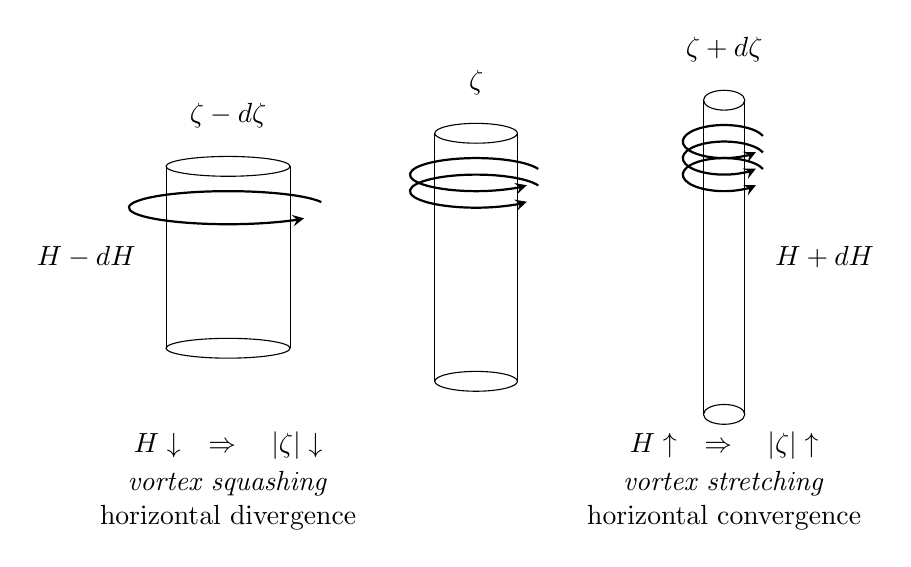
\begin{tikzpicture}[scale=1.05, >=stealth]
		% params
		\def\Rone{0.5}\def\Rtwo{0.25}\def\Rthree{0.75}\def\r{0.12}
		\def\H{3.0}  \def\dH{0.8}
		\def\DX{3}

		% guide rays (dashed perspective)
		% \draw[dashed] (-0.2,\H) -- (\DX+0.2,\H);
		% \draw[dashed] (-0.2,0)  -- (\DX+0.2,0);

		% center cylinder (height H)
		\draw (0,0) ellipse ({\Rone} and {\r});
		\draw (-\Rone,0) -- (-\Rone,\H);
		\draw (\Rone,0) -- (\Rone,\H);
		\draw (0,\H) ellipse ({\Rone} and {\r});
		\node[above] at (0,\H+0.35) {$\zeta$};
		% \draw[->] (1.4,1.7) -- (0.7,1.7);

		% right cylinder (H+dH)
		\begin{scope}[xshift=\DX cm]
			\draw (0,{-\dH/2}) ellipse ({\Rtwo} and {\r});         % bottom
			\draw (-\Rtwo,{-\dH/2}) -- (-\Rtwo,{\H+\dH/2});
			\draw ( \Rtwo,{-\dH/2}) -- ( \Rtwo,{\H+\dH/2});
			\draw (0,{\H+\dH/2}) ellipse ({\Rtwo} and {\r});        % top
			\node[above] at (0,{\H+\dH/2+0.35}) {$\zeta+d\zeta$};
			\node[right] at (\Rtwo+0.25,{\H/2}) {$H+dH$};  % center the label
			% \draw[->] (-1.4,{\H/2}) -- (-0.7,{\H/2});
		\end{scope}


		\begin{scope}[xshift={-\DX cm}]
			\draw (0,{ \dH/2}) ellipse ({\Rthree} and {\r});          % bottom
			\draw (-\Rthree,{ \dH/2}) -- (-\Rthree,{\H-\dH/2});
			\draw ( \Rthree,{ \dH/2}) -- ( \Rthree,{\H-\dH/2});
			\draw (0,{\H-\dH/2}) ellipse ({\Rthree} and {\r});        % top
			\node[above] at (0,{\H-\dH/2+0.35}) {$\zeta-d\zeta$};
			\node[left]  at (-\Rthree-0.25,{\H/2}) {$H-dH$}; % center the label
		\end{scope}
		% spin symbols on tops
		% spin symbols: use H±dH/2 so the midline matches
		% at the top (tweak to taste)
		\def\spinrxone{1.2}\def\spinrxtwo{0.8}\def\spinrxthree{0.5}
		\def\spinry{0.2}\def\spinstart{20}

		\foreach \x/\y/\spinrx in {-\DX/{\H-\dH/2}/\spinrxone, 0/{\H}/\spinrxtwo, \DX/{\H+\dH/2}/\spinrxthree}{
		\begin{scope}[xshift=\x cm]
			\draw[->, thick]
			({\spinrx*cos(\spinstart)}, {\y-0.5 + \spinry*sin(\spinstart)})
			arc[start angle=\spinstart, end angle=\spinstart+300,
					x radius=\spinrx, y radius=\spinry];
		\end{scope}
		}

		\foreach \x/\y/\spinrx in { 0/{\H}/\spinrxtwo, \DX/{\H+\dH/2}/\spinrxthree}{
		\begin{scope}[xshift=\x cm]
			\draw[->, thick]
			({\spinrx*cos(\spinstart)}, {\y-0.7 + \spinry*sin(\spinstart)})
			arc[start angle=\spinstart, end angle=\spinstart+300,
					x radius=\spinrx, y radius=\spinry];
		\end{scope}
		}

		\foreach \x/\y/\spinrx in { \DX/{\H+\dH/2}/\spinrxthree}{
		\begin{scope}[xshift=\x cm]
			\draw[->, thick]
			({\spinrx*cos(\spinstart)}, {\y-0.9 + \spinry*sin(\spinstart)})
			arc[start angle=\spinstart, end angle=\spinstart+300,
					x radius=\spinrx, y radius=\spinry];
		\end{scope}
		}

		% captions
		\node[align=center] at (-\DX,-1.2)
		{$H\downarrow \quad \Rightarrow \quad |\zeta|\downarrow$\\[2pt]\emph{vortex squashing}\\ horizontal divergence};
		\node[align=center] at (\DX,-1.2)
		{$H\uparrow \quad \Rightarrow \quad |\zeta|\uparrow$\\[2pt]\emph{vortex stretching}\\ horizontal convergence};
	\end{tikzpicture}
\end{document}
